\lab{Gibbs Sampling and LDA}{Gibbs Sampling and LDA}
\objective{Understand the basic principles of implementing a Gibbs sampler. Apply this to Latent Dirichlet Allocation.}

\section*{Gibbs Sampling}
Gibbs sampling is an MCMC sampling method in which we construct a Markov chain by which to sample from a desired joint (conditional) distribution
\begin{equation*}
\mathbb{P}(x_{1},\cdots,x_{n} | \mathbf{y}).
\end{equation*}
Often it is difficult to sample from this high-dimensional joint distribution, while it may be easy to sample from the one dimensional
conditional distributions
\begin{equation*}
\mathbb{P}(x_{i} | \mathbf{x}_{-i}, \mathbf{y})
\end{equation*}
where $\mathbf{x}_{-i} = x_{1},\cdots,x_{i-1},x_{i+1},\cdots,x_{n}.$

\begin{algorithm}
\begin{algorithmic}[1]
\Procedure{Gibbs Sampler}{}
    \State \textrm{Randomly initialize } $x_1,x_2,\ldots,x_n$.
    \For{$k = 1, 2, 3, \ldots$}
        \For{$i = 1, 2, \ldots,n$}
            \State \textrm{Draw } $x \sim \mathbb{P}(x_{i} | \mathbf{x}_{-i}, \mathbf{y})$
            \State \textrm{Fix } $x_i = x$
        \EndFor
        \State $\mathbf{x}^{(k)}= (x_1,x_2,\ldots,x_n)$
    \EndFor
\EndProcedure
\end{algorithmic}
\caption{Basic Gibbs Sampling Process.}
\label{alg:gibbs}
\end{algorithm}
A Gibbs sampler proceeds according to Algorithm \ref{alg:gibbs}.
Each iteration of the outer for-loop is a \emph{sweep} of the Gibbs sampler, and the value of $\mathbf{x}^{(k)}$ after a sweep is a sample. This creates an irreducible, non-null recurrent, aperiodic Markov chain over the state space consisting of all possible $\mathbf{x}$. The unique invariant distribution for the chain is the desired joint distribution
\begin{equation*}
\mathbb{P}(x_{1},\cdots,x_{n} | \mathbf{y}).
\end{equation*}
Thus, after a burn-in period, our samples $\mathbf{x}^{(k)}$ are effectively samples from the desired distribution.

Consider the data set of $N$ scores from a calculus exam in the file \texttt{examscores.csv}. We believe that the spread of these exam scores can be
modeled with a normal distribution of mean $\mu$ and variance $\sigma^{2}$.
Because we are unsure of the true value of $\mu$ and $\sigma^2$, we take a Bayesian approach and place priors on each parameter to quantify this uncertainty:
\begin{align*}
\mu & \sim N(\mu_{0}, \sigma_{0}^{2})\quad &&\text{(a normal distribution)} \\
\sigma^{2} & \sim IG(\alpha, \beta) &&\text{(an inverse gamma distribution)}
\end{align*}
Letting $\mathbf{y} = (y_1,\ldots,y_N)$ be the set of exam scores, we would like to update our beliefs of $\mu$ and $\sigma^2$ by sampling from the posterior
distribution
\begin{equation*}
\mathbb{P}(\mu, \sigma^{2} | \mathbf{y}, \mu_{0}, \sigma_{0}^{2}, \alpha, \beta).
\end{equation*}
Sampling directly can be difficult. However, we \emph{can} easily sample from the following conditional distributions:
\begin{align*}
\mathbb{P}(\mu | \sigma^{2}, \mathbf{y}, \mu_{0}, \sigma_{0}^{2}, \alpha, \beta) & = \mathbb{P}(\mu | \sigma^{2}, \mathbf{y}, \mu_{0}, \sigma_{0}^{2})\\
\mathbb{P}(\sigma^{2} | \mu, \mathbf{y}, \mu_{0}, \sigma_{0}^{2}, \alpha, \beta) & = \mathbb{P}(\sigma^{2} | \mu, \mathbf{y}, \alpha, \beta)
\end{align*}
The reason for this is that these conditional distributions are \emph{conjugate} to the prior distributions, and hence are part of the same distributional
families as the priors. In particular, we have
\begin{align*}
\mathbb{P}(\mu | \sigma^{2}, \mathbf{y}, \mu_{0}, \sigma_{0}^{2}) &= N(\mu^*, (\sigma^*)^2)\\
\mathbb{P}(\sigma^{2} | \mu, \mathbf{y}, \alpha, \beta) &= IG(\alpha^*, \beta^*),
\end{align*}
where
\begin{align*}
(\sigma^*)^2 &= \left(\frac{1}{\sigma_0^2}+\frac{N}{\sigma^2}\right)^{-1}\\
\mu^* &= (\sigma^*)^2\left(\frac{\mu_0}{\sigma_0^2} + \frac{1}{\sigma^2}\sum_{i=1}^N y_i \right)\\
\alpha^* &= \alpha + \frac{N}{2}\\
\beta^* &= \beta + \frac{1}{2}\sum_{i=1}^N (y_i-\mu)^2
\end{align*}
We have thus set this up as a Gibbs sampling problem, where we just have to alternate between sampling $\mu$ and $\sigma^{2}$.
We can sample from a normal distribution and an inverse gamma distribution as follows:
\begin{lstlisting}
>>> from math import sqrt
>>> from scipy.stats import norm
>>> from scipy.stats import invgamma
>>> mu = 0. # the mean
>>> sigma2 = 9. # the variance
>>> normal_sample = norm.rvs(mu, scale=sqrt(sigma))
>>> alpha = 2.
>>> beta = 15.
>>> invgamma_sample = invgamma.rvs(alpha, scale=beta)
\end{lstlisting}
Note that when sampling from the normal distribution, we need to set the \li{scale} parameter to the standard deviation, \emph{not} the variance.

\begin{problem}
Implement a Gibbs sampler for the exam scores problem using the following function declaration.
\begin{lstlisting}
def gibbs(y, mu0, sigma02, alpha, beta, n_samples):
    """
    Assuming a likelihood and priors
        y_i    ~ N(mu, sigma2),
        mu     ~ N(mu0, sigma02),
        sigma2 ~ IG(alpha, beta),
    sample from the posterior distribution
        P(mu, sigma2 | y, mu0, sigma02, alpha, beta)
    using a gibbs sampler.

    Parameters
    ----------
    y : ndarray of shape (N,)
        The data
    mu0 : float
        The prior mean parameter for mu
    sigma02 : float > 0
        The prior variance parameter for mu
    alpha : float > 0
        The prior alpha parameter for sigma2
    beta : float > 0
        The prior beta parameter for sigma2
    n_samples : int
        The number of samples to draw

    Returns
    -------
    samples : ndarray of shape (n_samples,2)
        1st col = mu samples, 2nd col = sigma2 samples
    """
    pass
\end{lstlisting}
Test it with priors $\mu_{0}=80, \sigma_{0}^{2} = 16, \alpha = 3, \beta = 50$, collecting $1000$ samples. Plot your samples of $\mu$ and your samples of $\sigma^{2}$. How long did it take for each to converge? It should have been very quick.
\end{problem}

We'd like to look at the posterior marginal distributions for $\mu$ and $\sigma^2$.
To plot these from the samples, we will use a kernel density estimator.
If our samples of $\mu$ are called \li{mu_samples}, then we can do this as follows:
\begin{lstlisting}
>>> import numpy as np
>>> from scipy.stats import gaussian_kde
>>> import matplotlib.pyplot as plt
>>> mu_kernel = gaussian_kde(mu_samples)
>>> x_min = min(mu_samples) - 1
>>> x_max = max(mu_samples) + 1
>>> x = np.arange(x_min, x_max, step=0.1)
>>> plt.plot(x,mu_kernel(x))
>>> plt.show()
\end{lstlisting}

\begin{figure}
	\begin{subfigure}[b]{.49\textwidth}
		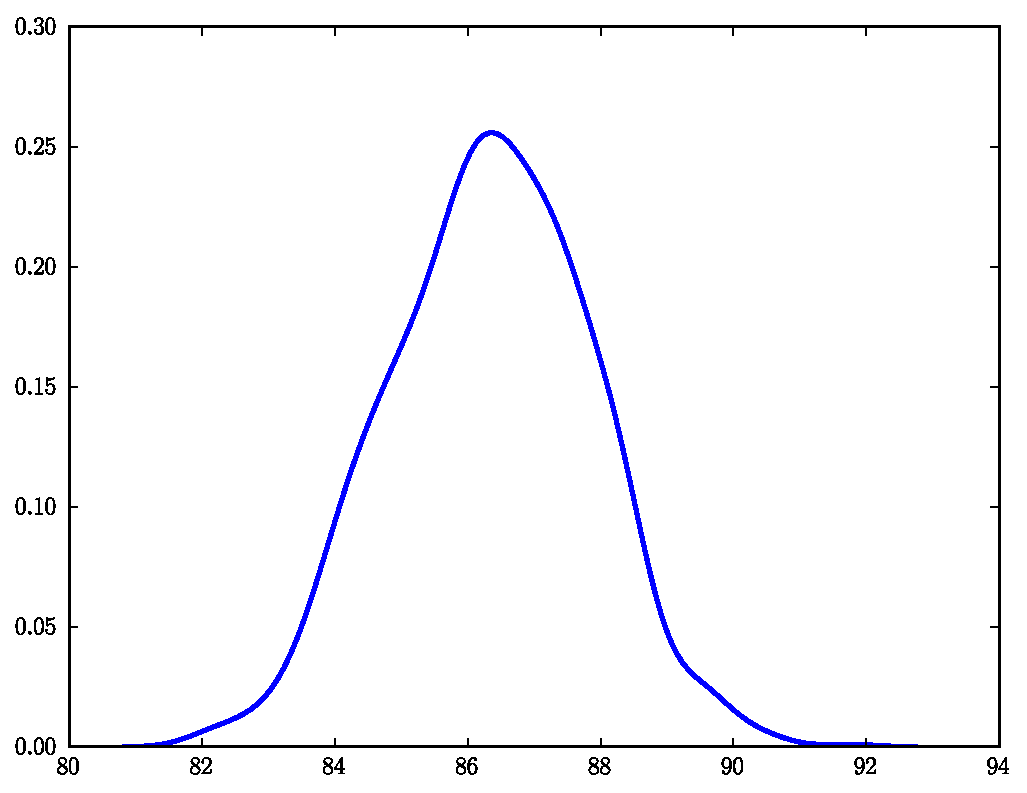
\includegraphics[width=\textwidth]{mu_posterior.pdf}
		\caption{Posterior distribution of $\mu$.}
	\end{subfigure}
	\begin{subfigure}[b]{.49\textwidth}
		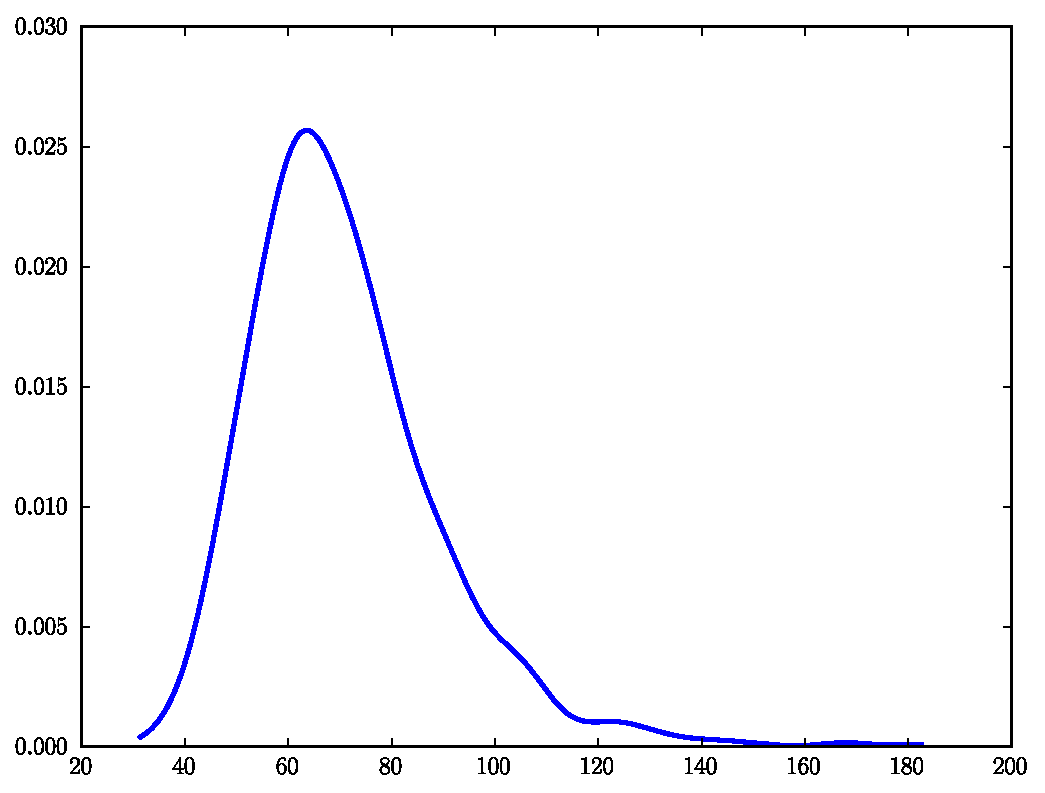
\includegraphics[width=\textwidth]{sigma2_posterior.pdf}
		\caption{Posterior distribution of $\sigma^2$.}
	\end{subfigure}
\caption{Posterior marginal probability densities for $\mu$ and $\sigma^2$.}
\label{fig:post}
\end{figure}

\begin{problem}
Plot the kernel density estimators for the posterior distributions of $\mu$ and $\sigma^{2}$.
You should get plots similar to those in Figure \ref{fig:post}.
\end{problem}

Keep in mind that the above plots are of the posterior distributions of the \emph{parameters}, not of the scores. If we would like to compute the posterior distribution of a new exam score $\tilde{y}$ given our data $\mathbf{y}$ and prior parameters, we compute what is known as the \emph{posterior predictive distribution}:
\begin{equation*}
\mathbb{P}(\tilde{y} | \mathbf{y}, \lambda) = \int_{\Theta} \mathbb{P}(\tilde{y} | \Theta)\mathbb{P}(\Theta | \mathbf{y}, \lambda) d\Theta
\end{equation*}
where $\Theta$ denotes our parameters (in our case $\mu$ and $\sigma^{2}$) and $\lambda$ denotes our prior parameters (in our case $\mu_{0}, \sigma_{0}^{2}, \alpha,$ and $\beta$).

Rather than actually computing this integral for each possible $\tilde{y}$, we can do this by sampling scores from our parameter samples. In other words, sample
\begin{equation*}
\tilde{y}_{(t)} \sim N(\mu_{(t)}, \sigma_{(t)}^{2})
\end{equation*}
for each sample pair $\mu_{(t)}, \sigma_{(t)}^{2}$. Now we have essentially drawn samples from our posterior predictive distribution, and we can use a kernel density estimator to plot this distribution from the samples.

\begin{figure}
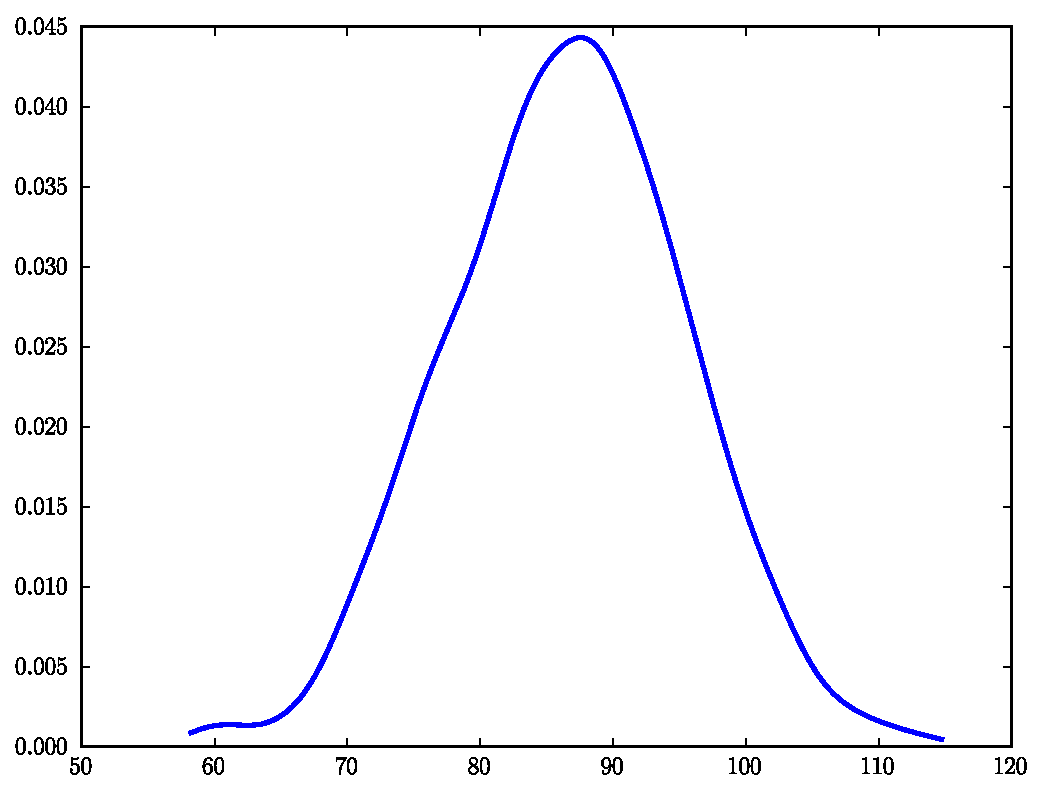
\includegraphics[width=\textwidth]{predictiveposterior.pdf}
\caption{Predictive posterior distribution of exam scores.}
\label{fig:predictive}
\end{figure}

\begin{problem}
Use your samples to draw samples from the posterior predictive distribution. Plot the kernel density estimator of your sampled scores.
It should resemble the plot in Figure \ref{fig:predictive}.
\end{problem}

\section*{Latent Dirichlet Allocation}
Gibbs sampling can be applied to an interesting problem in language processing: that of determining which topics are prevalent in a document.
Latent Dirichlet Allocation (LDA) is a generative model for a collection of text documents.
It supposes that there is some fixed vocabulary of terms (of length $V$) and $K$ different topics, each represented as a probability distribution $\phi_{k}$ over the vocabulary, each with a Dirichlet prior $\beta$.
With the vocabulary and topics chosen, the LDA model assumes that a set of $D$ documents is generated as follows.
The $m$-th document consists of $N_m$ words, and
a probability distribution $\theta_{m}$ over the topics is drawn from a Dirichlet distribution with parameter $\alpha$.
To generate each new word in the $m$-th document, we first draw a topic assignment $z_{m,n}$ from the categorical distribution $\theta_{m}$, and then we draw a word $w_{m,n}$ from the categorical distribution $\phi_{z_{m,n}}$. Throughout this implementation, we assume $\alpha$ and $\beta$ are scalars. In summary, we have
\begin{enumerate}
	\item Draw $\phi_{k} \sim \text{Dir}(\beta)$ for $1 \leq k \leq K$.
	\item For $1 \leq m \leq D$:
	\begin{enumerate}
        \item Draw $\theta_{m} \sim \text{Dir}(\alpha)$.
        \item Draw $z_{m,n} \sim \text{Cat}(\theta_{m})$ for $1 \leq n \leq N_{m}$.
	    \item Draw $w_{m,n} \sim \text{Cat}(\phi_{z_{m,n}})$ for $1 \leq n \leq N_{m}$.
	\end{enumerate}
\end{enumerate}
This is typically depicted with graphical plate notation as in Figure \ref{fig:ldaplates}.
\begin{figure}[h]
\centering
\begin{tikzpicture}[>=stealth', dot/.style=
	{circle,fill=black,minimum size=3pt,inner sep=0pt, outer sep=-1pt} ]

\node[draw,minimum height=3.2cm, minimum width=2.1cm](r1)[]{};
\node[draw,minimum height=5cm, minimum width=2.4cm, node distance=
	.4cm](r2)[above of=r1]{};

\node[node distance=1.3cm](Nm)[below of=r1]{$1 \le n \le N_m$};
\node[node distance=2.28cm](M)[below of=r2]{$1 \le m \le M$};

\node[node distance = 2.7cm](dummy3)[left of=r1]{};
\node[draw,minimum height=2cm, minimum width=2.1cm, node distance=
	.55cm](r3)[ below of =dummy3]{};
\node[node distance=.7cm](K)[below of=r3]{$1 \le k \le K$};

\node[node distance=.6cm](dummy)[above right of =Nm]{};
\node[circle, draw,  inner sep=1pt, fill=black!25!,node distance=.4cm]
	(w)[above of=dummy]{$w_{m,n}$};
\node[circle, draw,  inner sep=1pt, node distance=1.3cm](z)[above
	of=w]{$z_{m,n}$};
\node[circle, draw,  inner sep=1pt, node distance=1.3cm]
	(theta)[above of=z]{$\vec{\theta}_{m}$};

\node[node distance=1.2cm, inner sep=0pt](alpha)[above of=
	theta]{$\vec{\alpha}$};

\node[node distance=.6cm](dummy2)[above right of=K]{};
\node[node distance=.35cm, circle, inner sep=1pt, draw](phi)[above
	of=dummy2]{$\vec{\phi_k}$};
\node[node distance=1.4cm, inner sep=0pt](beta)[above of = phi]{$\vec{\beta}$};

\foreach \x/\y in {alpha/theta, theta/z, z/w, beta/phi, phi/w} \draw[->](\x)--(\y);

\end{tikzpicture}
\caption{Graphical plate notation for LDA text generation.}
\label{fig:ldaplates}
\end{figure}

In the plate model, only the variables $w_{m,n}$ are shaded, signifying that these are the only observations visible to us; the rest are latent variables. Our goal is to estimate each $\phi_{k}$ and each $\theta_{m}$. This will allow us to understand what each topic is, as well as understand how each document is distributed over the $K$ topics. We can estimate these well if we know $z_{m,n}$ for each $m, n$, collectively referred to as $\mathbf{z}$. Thus, we need to sample
$\mathbf{Z}$ from the posterior distribution $\mathbb{P}(\mathbf{z} | \mathbf{w}, \alpha, \beta),$ where $\mathbf{w}$ is the collection words in the text corpus. Unsurprisingly, it is intractable to sample directly from the joint posterior distribution. However, letting $\mathbf{z}_{\neg (m,n)} = \mathbf{z}\setminus \{z_{m,n}\}$, the conditional posterior distributions
\[\mathbb{P}(z_{m,n} = k | \mathbf{z}_{\neg (m,n)}, \mathbf{w}, \alpha, \beta)\]
have nice, closed form solutions, making them easy to sample from.

These conditional distributions have the following form:
\begin{equation*}
\mathbb{P}(z_{m,n} = k | \mathbf{z}_{\neg (m,n)}, \mathbf{w}, \alpha, \beta) \propto \frac{(n_{(k,m,\cdot)}^{\neg (m,n)} + \alpha)(n_{(k, \cdot, w_{m,n})}^{\neg (m,n)} + \beta)}{n_{(k,\cdot,\cdot)}^{\neg (m,n)} + V \beta}
\end{equation*}
where
\begin{align*}
n_{(k,m,\cdot)} & = \mbox{ the number of words in document $m$ assigned to topic $k$} \\
n_{(k,\cdot,v)} & = \mbox{ the number of times term $v = w_{m,n}$ is assigned to topic $k$} \\
n_{(k,\cdot,\cdot)} & = \mbox{ the number of times topic $k$ is assigned in the corpus} \\
n_{(k,m,\cdot)}^{\neg (m,n)} & = n_{(k,m,\cdot)} - \indicator{z_{m,n} = k} \\
n_{(k,\cdot,v)}^{\neg (m,n)} & = n_{(k,\cdot,v)} - \indicator{z_{m,n} = k} \\
n_{(k,\cdot,\cdot)}^{\neg (m,n)} & = n_{(k,\cdot,\cdot)} - \indicator{z_{m,n} = k}
\end{align*}

Thus, if we simply keep track of these count matrices, then we can easily create a Gibbs sampler over the topic assignments. This is actually a particular class of samplers known as \emph{collapsed Gibbs samplers}, because we have collapsed the sampler by integrating out $\theta$ and $\phi$.

We have provided for you the structure of a Python object \li{LDACGS} with several methods. The object is already defined to have attributes \li{n\_topics}, \li{documents}, \li{vocab}, \li{alpha}, and \li{beta}, where \li{vocab} is a list of strings (terms), and documents is a list of dictionaries (a dictionary for each document). Each entry in dictionary $m$ is of the form $n : w$, where $w$ is the index in \li{vocab} of the $n^{th}$ word in document $m$.

Throughout this lab we will guide you through writing several more methods in order to implement the Gibbs sampler. The first step is to initialize our assignments, and create the count matrices $n_{(k,m,\cdot)}, n_{(k,\cdot,v)}$ and vector $n_{(k,\cdot,\cdot)}$.

\begin{problem}
Complete the method \li{initialize}. By randomly assigning initial topics, fill in the count matrices and topic assignment dictionary. In this method, you will initialize the count matrices (among other things). Note that the notation
provided in the code is slightly different than that used above. Be sure to understand how the formulae above
connect with the code.
\end{problem}

The next method we need to write fully outlines a sweep of the Gibbs sampler.

\begin{problem}
Complete the method \li{\_sweep}, which needs to iterate through each word of each document. It should call on the method \li{\_conditional} to get the conditional distribution at each iteration.
\end{problem}

\begin{comment}
Take out this problem to make the lab easier.
We need to write the method to create the appropriate conditional distribution.

\begin{problem}
Complete the method \li{\_conditional}. It accepts arguments $m,w$ where $m$ is the document and $w$ is an index of \li{vocab}. Don't forget to normalize to ensure you are actually returning a distribution!
\end{problem}
\end{comment}
We are now prepared to write the full Gibbs sampler.

\begin{problem}
Complete the method \li{sample}. The argument \emph{filename} is the name and location of a .txt file, where each line is considered a document. The corpus is built by method \li{buildCorpus}, and stopwords are removed (if argument \emph{stopwords} is provided). Burn in the Gibbs sampler, computing and saving the log-likelihood with the method \li{\_loglikelihood}. After the burn in, iterate further, accumulating your count matrices, by adding \li{nzw} and \li{nmz} to \li{total\_nzw} and \li{total\_nmz} respectively, where you only add every \emph{sample\_rate}$^{th}$ iteration. Also save each log-likelihood.
\end{problem}

You should now have a working Gibbs sampler to perform LDA inference on a corpus. Let's test it out on Ronald Reagan's State of the Union addresses.

\begin{problem}
Create an \li{LDACGS} object with $20$ topics, letting \li{alpha} and \li{beta} be the default values. Load in the stop word list provided. Run the Gibbs sampler, with a burn in of $100$ iterations, accumulating $10$ samples, only keeping the results of every $10$ sweep. Plot the log-likelihoods. How long did it take to truly burn in?
\end{problem}

We can estimate the values of each $\phi_{k}$ and each $\theta_{m}$ as follows:

\begin{align*}
\widehat{\theta}_{m,k} & = \frac{n_{(k,m,\cdot)} + \alpha}{K \cdot \alpha + \sum_{k=1}^{K} n_{(k,m,\cdot)}} \\
\widehat{\phi}_{k,v} & = \frac{n_{(k,\cdot,v)} + \beta}{V \cdot \beta + \sum_{v=1}^{V} n_{(k,\cdot,v)}}
\end{align*}

We have provided methods \li{phi} and \li{theta} that do this for you. We often examine the topic-term distributions $\phi_{k}$ by looking at the $n$ terms with highest probability, where $n$ is small (say $10$ or $20$).  We have provided a method \li{topterms} which does this for you.

\begin{problem}
Using the methods described above, examine the topics for Reagan's addresses. As best as you can, come up with labels for each topic.
\end{problem}

We can use $\widehat{\theta}$ to find the paragraphs in Reagan's addresses that focus the most on each topic. The documents with highest values of $\widehat{\theta}_{k}$ are those most heavily focused on topic $k$.

\begin{problem}
In your above topic analysis, you should have found a topic about the Cold War and one about education. Find the five paragraphs in Reagan's addresses that most closely focus on each of these topics, according to the above method.
\end{problem}
